Stabilität Sphere:
\textbf{WHATWHATWHATWHATWHATWHATWHATWHATWHAT}
\begin{figure}
  \centering
  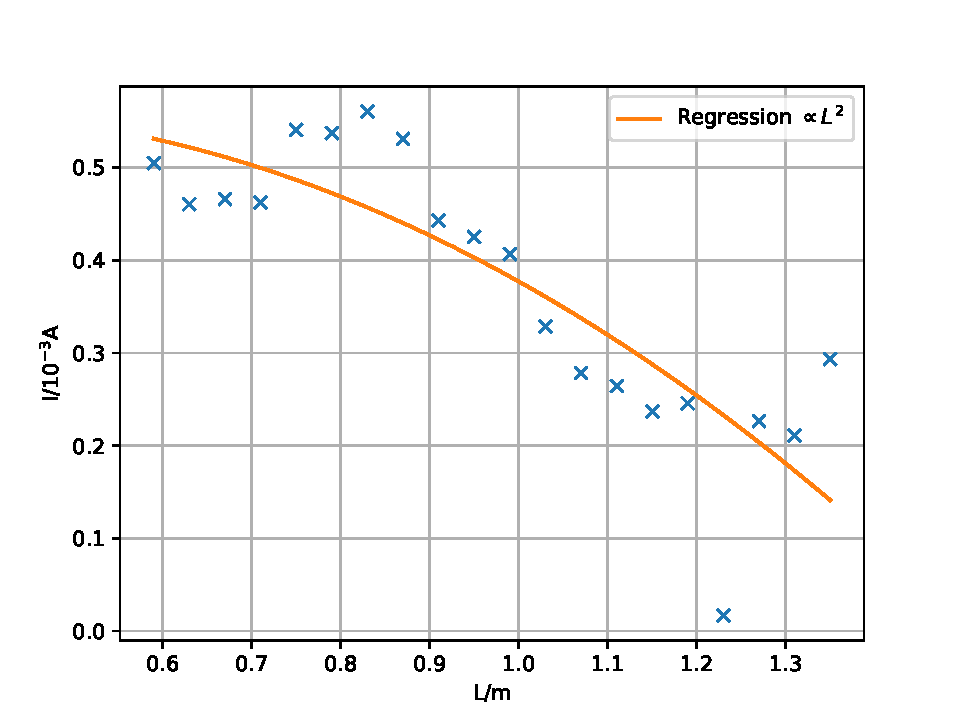
\includegraphics[width=0.8\textwidth]{stabsphere.pdf}
  \caption{Überprüfung der Stabilitätsbedingung beim doppeltsphärischen Aufbau}
  \label{fig:stabsphere}
\end{figure}
Fit:
\begin{equation*}
  I= \frac{a(L+b)^2}{r_1 r_2}+\frac{c(L+d)}{r_1 r_2}+\frac{e}{r_1 r_2}
\end{equation*}
\FloatBarrier
\begin{align*}
a &=& \SI{0.77019576  \pm 6.67239536e-01}{} \\
b &=& \SI{0.68148470  \pm 5.70376283e+12}{} \\
c &=& \SI{-1.53874317 \pm 1.35339234e+13}{} \\
d &=& \SI{2.97459567  \pm 1.52142773e+13}{} \\
e &=& \SI{3.19916773  \pm 1.03956309e+12}{} \\
\end{align*}
\FloatBarrier

Stabilität Flat:
\begin{figure}
  \centering
  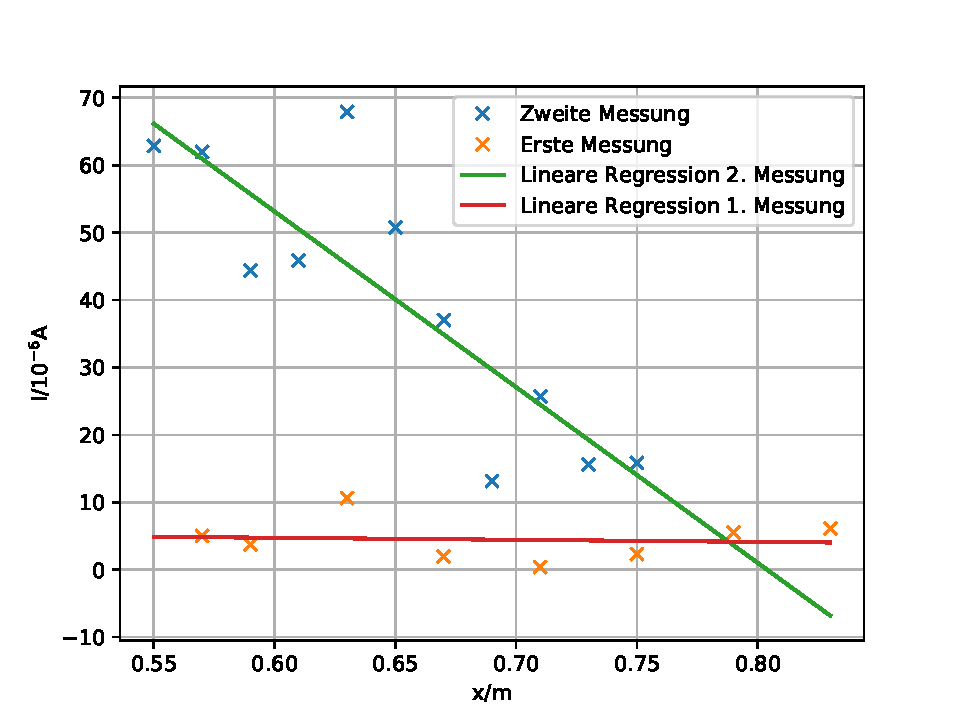
\includegraphics[width=0.8\textwidth]{stabflat.pdf}
  \caption{Überprüfung der Stabilitätsbedingung beim flach-sphärischen Aufbau}
  \label{fig:stabflat}
\end{figure}
Fit:
\begin{equation*}
  I= aL+b
\end{equation*}
\FloatBarrier
\begin{align*}
&&\text{zweite Messung} \\
a &=& \SI{260.60636539 \pm 2739.59243164}{} \\
b &=& \SI{-209.49268296 \pm 1168.43618691}{} \\
&&\text{erste Messung} \\
a &=& \SI{3.03299421 \pm 187.11756018}{} \\
b &=& \SI{-6.55319099 \pm 91.18238783}{} \\
\end{align*}
\FloatBarrier

Grundmode:
\begin{figure}
  \centering
  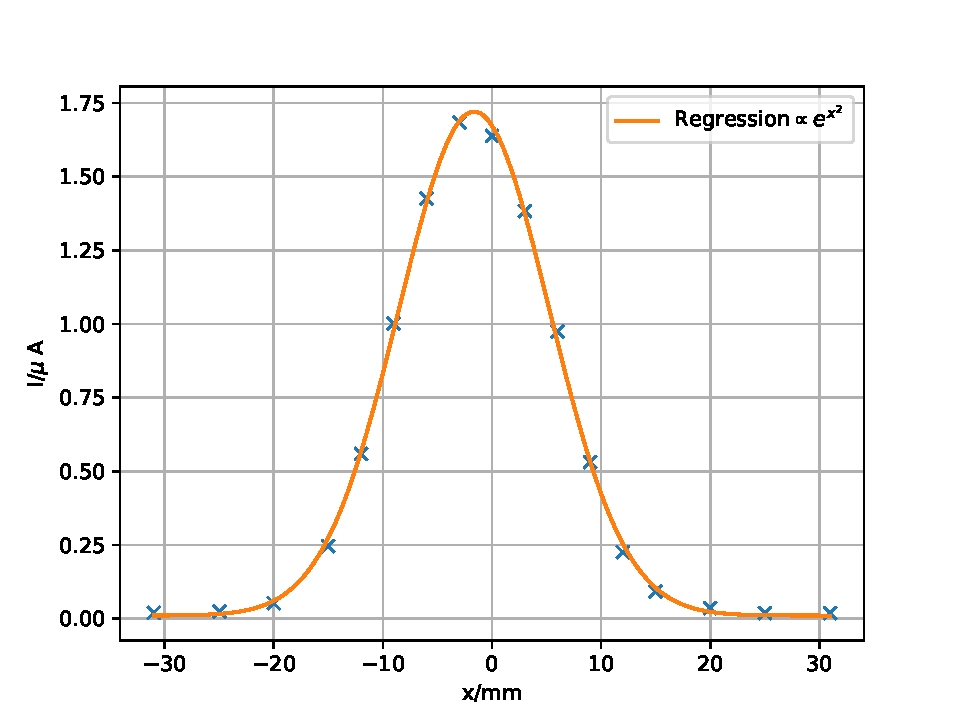
\includegraphics[width=0.8\textwidth]{grundmode.pdf}
  \caption{Intensitätsverteilung der Grundmode}
  \label{fig:grundmode}
\end{figure}
Fit:
\begin{equation*}
  I= a \exp{\left( b(x-c)^2 \right)}+d
\end{equation*}
\begin{align*}
a &=& \SI{ 1.71042307 \pm 2.01428259e-04}{}\\
b &=& \SI{-0.01047146 \pm 5.10717911e-08}{}\\
c &=& \SI{-1.64149566 \pm 3.45206452e-03}{}\\
d &=& \SI{ 0.01007865 \pm 7.33843461e-05}{}\\
\end{align*}
\FloatBarrier

Erste Mode:
\begin{align*}
kommt noch\\
\end{align*}
\FloatBarrier
